% author:   sam tenka
% change:   2022-05-28
% create:   2022-05-11

%==============================================================================
%====  0.  DOCUMENT SETTINGS  ================================================
%==============================================================================

%~~~~~~~~~~~~~~~~~~~~~~~~~~~~~~~~~~~~~~~~~~~~~~~~~~~~~~~~~~~~~~~~~~~~~~~~~~~~~~
%~~~~~~~~~~~~~  0.0. About this Exposition  ~~~~~~~~~~~~~~~~~~~~~~~~~~~~~~~~~~~

%---------------------  0.0.0. page geometry  ---------------------------------
\documentclass[11pt, justified]{tufte-book}
\geometry{
  left           = 0.90in, % left margin
  textwidth      = 4.95in, % main text block
  marginparsep   = 0.15in, % gutter between main text block and margin notes
  marginparwidth = 2.30in, % width of margin notes
                 % 0.20in  % width from margin to edge
}

%---------------------  0.0.1. math packages  ---------------------------------
\newcommand\hmmax{0} % to allow for more fonts 
\newcommand\bmmax{0} % to allow for more fonts
\usepackage{amsmath, amssymb, amsthm, mathtools}
\usepackage{bm}
\usepackage{euler}

\usepackage{array}   % for \newcolumntype macro
\newcolumntype{L}{>{$}l<{$}} % math-mode version of "l" column type
\newcolumntype{C}{>{$}c<{$}} % math-mode version of "c" column type
\newcolumntype{R}{>{$}r<{$}} % math-mode version of "r" column type

%---------------------  0.0.2. graphics packages  -----------------------------
\usepackage{graphicx, xcolor}
\usepackage{float, capt-of}

%---------------------  0.0.3. packages for fancy text  -----------------------
\usepackage{enumitem}\setlist{nosep}
\usepackage{listings}
\usepackage{xstring}
\usepackage{fontawesome5}

%---------------------  0.043. colors  ----------------------------------------
\definecolor{mblu}{rgb}{0.05, 0.35, 0.70} \newcommand{\blu}{\color{mblu}}
\definecolor{mbre}{rgb}{0.30, 0.45, 0.60} \newcommand{\bre}{\color{mbre}}
\definecolor{mbro}{rgb}{0.60, 0.05, 0.05} \newcommand{\bro}{\color{mbro}}
\definecolor{mcya}{rgb}{0.10, 0.45, 0.45} \newcommand{\cya}{\color{mcya}}
\definecolor{mgre}{rgb}{0.55, 0.55, 0.50} \newcommand{\gre}{\color{mgre}}
\definecolor{mgrn}{rgb}{0.15, 0.65, 0.05} \newcommand{\grn}{\color{mgrn}}
\definecolor{mred}{rgb}{0.90, 0.05, 0.05} \newcommand{\red}{\color{mred}}

%~~~~~~~~~~~~~~~~~~~~~~~~~~~~~~~~~~~~~~~~~~~~~~~~~~~~~~~~~~~~~~~~~~~~~~~~~~~~~~
%~~~~~~~~~~~~~  0.1. Headers and References  ~~~~~~~~~~~~~~~~~~~~~~~~~~~~~~~~~~

%---------------------  0.1.0. intra-document references  ---------------------
\newcommand{\offour}[1]{
    {\tiny \raisebox{0.04cm}{\scalebox{0.9}{$\substack{
        \IfSubStr{#1}{0}{{\blacksquare}}{\square}   
        \IfSubStr{#1}{1}{{\blacksquare}}{\square} \\ 
        \IfSubStr{#1}{2}{{\blacksquare}}{\square}   
        \IfSubStr{#1}{3}{{\blacksquare}}{\square}   
    }$}}}%
}

\newcommand{\offourline}[1]{
    {\tiny \raisebox{0.04cm}{\scalebox{0.9}{$\substack{
        \IfSubStr{#1}{0}{{\blacksquare}}{\square}   
        \IfSubStr{#1}{1}{{\blacksquare}}{\square}
        \IfSubStr{#1}{2}{{\blacksquare}}{\square}   
        \IfSubStr{#1}{3}{{\blacksquare}}{\square}   
    }$}}}%
}
\newcommand{\notesam}[1]{{\blu \textsf{#1}}}
\newcommand{\attn}[1]{{\bro \textsf{#1}}}
\newcommand{\attnsam}[1]{{\red \textsf{#1}}}

\newcommand{\blarr}{\hspace{-0.15cm}${\bro \leftarrow}\,$}
\newcommand{\bcirc}{${\bro ^\circ}$}

\newcounter{footprintssofar}
\setcounter{footprintssofar}{90}
\newcommand{\plainfootprint}{{\bro \rotatebox{\value{footprintssofar}}{\faIcon{shoe-prints}}}\setcounter{footprintssofar}{\value{footprintssofar}+30} }
\newcommand{\footprint}{\marginnote{\plainfootprint} }

%---------------------  0.1.1. table of contents helpers  ---------------------
\newcommand{\phdot}{\phantom{.}}

%---------------------  0.1.2. section headers  -------------------------------
\newcommand{\samtitle} [1]{
  \par\noindent{\Huge \sf \blu #1}
  \vspace{0.4cm}
}

\newcommand{\samquote} [2]{
    \marginnote[-0.4cm]{\begin{flushright}
    \scriptsize
        \gre {\it #1} \\ --- #2
    \end{flushright}}
}

\newcommand{\samsection} [1]{
  \vspace{0.5cm}
  \par\noindent{\LARGE \sf \blu #1}
  \vspace{0.1cm}\par
}

\newcommand{\samsubsection}[1]{
  \vspace{0.3cm}
  \par\noindent{\Large \sf \bre #1}
  \vspace{0.1cm}\par
}

\newcommand{\samsubsubsection}[1]{
   \vspace{0.1cm}
   \par\noindent{\hspace{-2cm}\normalsize \sc \gre #1} ---
}

%---------------------  0.1.3. clear the bibliography's header  ---------------
\usepackage{etoolbox}
\patchcmd{\thebibliography}{\section*{\refname}}{}{}{}

%~~~~~~~~~~~~~~~~~~~~~~~~~~~~~~~~~~~~~~~~~~~~~~~~~~~~~~~~~~~~~~~~~~~~~~~~~~~~~~
%~~~~~~~~~~~~~  0.2. Math Symbols and Blocks  ~~~~~~~~~~~~~~~~~~~~~~~~~~~~~~~~~

%---------------------  0.2.0. general math operators  ------------------------
\newcommand{\scirc}{\mathrel{\mathsmaller{\mathsmaller{\mathsmaller{\circ}}}}}
\newcommand{\cmop}[2]{{(#1\!\to\!#2)}}

%---------------------  0.2.1. probability symbols  ---------------------------
\newcommand{\KL}{\text{KL}}
\newcommand{\EN}{\text{H}}
\newcommand{\note}[1]{{\blu \textsf{#1}}}

%---------------------  0.2.2. losses averaged in various ways  ---------------
\newcommand{\Ein}  {\text{trn}_{\sS}}
\newcommand{\Einb} {\text{trn}_{\check\sS}}
\newcommand{\Einc} {\text{trn}_{\sS\sqcup \check\sS}}
\newcommand{\Egap} {\text{gap}_{\sS}}
\newcommand{\Eout} {\text{tst}}

%---------------------  0.2.3. double-struck and caligraphic upper letters  ---
\newcommand{\Aa}{\mathbb{A}}\newcommand{\aA}{\mathcal{A}}
\newcommand{\Bb}{\mathbb{B}}\newcommand{\bB}{\mathcal{B}}
\newcommand{\Cc}{\mathbb{C}}\newcommand{\cC}{\mathcal{C}}
\newcommand{\Dd}{\mathbb{D}}\newcommand{\dD}{\mathcal{D}}
\newcommand{\Ee}{\mathbb{E}}\newcommand{\eE}{\mathcal{E}}
\newcommand{\Ff}{\mathbb{F}}\newcommand{\fF}{\mathcal{F}}
\newcommand{\Gg}{\mathbb{G}}\newcommand{\gG}{\mathcal{G}}
\newcommand{\Hh}{\mathbb{H}}\newcommand{\hH}{\mathcal{H}}
\newcommand{\Ii}{\mathbb{I}}\newcommand{\iI}{\mathcal{I}}
\newcommand{\Jj}{\mathbb{J}}\newcommand{\jJ}{\mathcal{J}}
\newcommand{\Kk}{\mathbb{K}}\newcommand{\kK}{\mathcal{K}}
\newcommand{\Ll}{\mathbb{L}}\newcommand{\lL}{\mathcal{L}}
\newcommand{\Mm}{\mathbb{M}}\newcommand{\mM}{\mathcal{M}}
\newcommand{\Nn}{\mathbb{N}}\newcommand{\nN}{\mathcal{N}}
\newcommand{\Oo}{\mathbb{O}}\newcommand{\oO}{\mathcal{O}}
\newcommand{\Pp}{\mathbb{P}}\newcommand{\pP}{\mathcal{P}}
\newcommand{\Qq}{\mathbb{Q}}\newcommand{\qQ}{\mathcal{Q}}
\newcommand{\Rr}{\mathbb{R}}\newcommand{\rR}{\mathcal{R}}
\newcommand{\Ss}{\mathbb{S}}\newcommand{\sS}{\mathcal{S}}
\newcommand{\Tt}{\mathbb{T}}\newcommand{\tT}{\mathcal{T}}
\newcommand{\Uu}{\mathbb{U}}\newcommand{\uU}{\mathcal{U}}
\newcommand{\Vv}{\mathbb{V}}\newcommand{\vV}{\mathcal{V}}
\newcommand{\Ww}{\mathbb{W}}\newcommand{\wW}{\mathcal{W}}
\newcommand{\Xx}{\mathbb{X}}\newcommand{\xX}{\mathcal{X}}
\newcommand{\Yy}{\mathbb{Y}}\newcommand{\yY}{\mathcal{Y}}
\newcommand{\Zz}{\mathbb{Z}}\newcommand{\zZ}{\mathcal{Z}}

%---------------------  0.2.4. sans serif and frak lower letters  -------------
\newcommand{\sfa}{\mathsf{a}}\newcommand{\fra}{\mathcal{a}}
\newcommand{\sfb}{\mathsf{b}}\newcommand{\frb}{\mathcal{b}}
\newcommand{\sfc}{\mathsf{c}}\newcommand{\frc}{\mathcal{c}}
\newcommand{\sfd}{\mathsf{d}}\newcommand{\frd}{\mathcal{d}}
\newcommand{\sfe}{\mathsf{e}}\newcommand{\fre}{\mathcal{e}}
\newcommand{\sff}{\mathsf{f}}\newcommand{\frf}{\mathcal{f}}
\newcommand{\sfg}{\mathsf{g}}\newcommand{\frg}{\mathcal{g}}
\newcommand{\sfh}{\mathsf{h}}\newcommand{\frh}{\mathcal{h}}
\newcommand{\sfi}{\mathsf{i}}\newcommand{\fri}{\mathcal{i}}
\newcommand{\sfj}{\mathsf{j}}\newcommand{\frj}{\mathcal{j}}
\newcommand{\sfk}{\mathsf{k}}\newcommand{\frk}{\mathcal{k}}
\newcommand{\sfl}{\mathsf{l}}\newcommand{\frl}{\mathcal{l}}
\newcommand{\sfm}{\mathsf{m}}\newcommand{\frm}{\mathcal{m}}
\newcommand{\sfn}{\mathsf{n}}\newcommand{\frn}{\mathcal{n}}
\newcommand{\sfo}{\mathsf{o}}\newcommand{\fro}{\mathcal{o}}
\newcommand{\sfp}{\mathsf{p}}\newcommand{\frp}{\mathcal{p}}
\newcommand{\sfq}{\mathsf{q}}\newcommand{\frq}{\mathcal{q}}
\newcommand{\sfr}{\mathsf{r}}\newcommand{\frr}{\mathcal{r}}
\newcommand{\sfs}{\mathsf{s}}\newcommand{\frs}{\mathcal{s}}
\newcommand{\sft}{\mathsf{t}}\newcommand{\frt}{\mathcal{t}}
\newcommand{\sfu}{\mathsf{u}}\newcommand{\fru}{\mathcal{u}}
\newcommand{\sfv}{\mathsf{v}}\newcommand{\frv}{\mathcal{v}}
\newcommand{\sfw}{\mathsf{w}}\newcommand{\frw}{\mathcal{w}}
\newcommand{\sfx}{\mathsf{x}}\newcommand{\frx}{\mathcal{x}}
\newcommand{\sfy}{\mathsf{y}}\newcommand{\fry}{\mathcal{y}}
\newcommand{\sfz}{\mathsf{z}}\newcommand{\frz}{\mathcal{z}}

%---------------------  0.2.5. math environments  -----------------------------
\newtheorem*{qst}{Question}
\newtheorem*{thm}{Theorem}
\newtheorem*{lem}{Lemma}
% ...
\theoremstyle{definition}
\newtheorem*{dfn}{Definition}

%==============================================================================
%=====  1.  PROLOGUE  =========================================================
%==============================================================================

\begin{document}
\samtitle{recitation 02 (optional 6.86x notes)}

      \attn{You do not need to read these notes at all} to get an A
      in this course; conversely, \attn{you may not cite these notes} when
      solving homework or exams.
       
%==============================================================================
%=====  2.  LINEAR MODELS  ====================================================
%==============================================================================

  \samsection{B. linear models: the basics}
    \samsubsection{linear approximations} 
      \samquote{
        He had bought a large map representing the sea, \\
        Without the least vestige of land: \\
        And the crew were much pleased when they found it to be \\
        A map they could all understand.
      }{charles dodgson}
      \samsubsubsection{featurization}  % as an art of 
        As in the prologue, we represent our input $x$ as a fixed-length list
        of numbers so that we can treat $x$ with math. % \footprint There, we
        represented each photograph by $2$ numbers: height and darkness.  We
        could instead have represented each photograph by $784$ numbers, one
        for the brightness at each of the $28\cdot 28=784$ many pixels.  Or by
        $10$ numbers, each measuring the overlap of $x$'s ink with that of
        ``representative'' photos of the digits $0$ through $9$.

        When we choose how to represent $x$ by a list of numbers, %\footprint
        we're
        choosing a \textbf{featurization}.  We call each number a ``feature''.
        For example, height and darkness are two features.

        %``height'' and ``darkness'' are \emph{features}: maps $\xX\to \Rr$ used
        %to pre-process $x$s.

        \attnsam{TODO: mention one-hot, etc}
        \attnsam{TODO: mention LOWRANK (sketching; also, for multiregression)}
        %
        There are lots of interesting featurizations, each making different
        patterns easier to learn.\marginnote{%
            \attnsam{data-based featurizations via kernels}
            \attnsam{will soon learn featurizations}
            \attnsam{hand featurization in kaggle and medicine}
        }
        So we judge a featurization with respect to
        the kinds of patterns we use it to learn. %\footprint
        \attnsam{TODO: graphic of separability; and how projection can reduce it}
        Learning usually happens
        more accurately, robustly, and interpretably when our featurization is
        abstract (no irrelevant details) but complete (all relevant details),
        compressed (hard to predict one feature from the others) but accessible
        (easy to compute interesting properties from features).

        \attnsam{TODO: projectivization (say this foreshadows kernel discussion?)}

        %In the exercise at the end of the passage on ``meeting the data'', we
        %dreamed up other ``features'' (besides \emph{height} and
        %\emph{darkness}) that might help to distinguish ${\red{9}}$s
        %from ${\cya{1}}$s.
        %%
        %Maybe we thought of \emph{width}.  Or of whether the ink surrounds a
        %\emph{hole}, as in a ${\red{9}}$.  Or of a photo's \emph{topheaviness}:
        %is its top half darker than its bottom half?  We might have chosen a
        %`canonical' photo of each of the digits in order to consider how a
        %given photo's ink \emph{overlaps} with those canonical photos'.
        %%
        %These are just some of very many good ideas.

        %Let's crudely define a photo as having a \emph{hole} at location
        %$(r,c)$ when, for each quadrant around $(r, c)$, location
        %$(r,c)$ is strictly brighter than a location in that quadrant.  A
        %photo's \emph{holiness} is the fraction of its pixels that are holes.

        %And let's define the \emph{overlap} between two photos as the fraction
        %of their pixels that are both above or both below $0.5$ in darkness.  

        %\begin{lstlisting}[language=Python, basicstyle=\footnotesize\ttfamily]
        %  SIDE = 28
        %  def darkness(x):
        %    return np.mean(np.mean(x))
        %  def height(x):
        %    return np.std([row for col in range(SIDE)
        %                       for row in range(SIDE)
        %                       if 0.5 < x[row][col]  ])/(SIDE/2.0) 
        %  def width(x):
        %    return np.std([row for col in range(SIDE)
        %                       for row in range(SIDE)
        %                       if 0.5 < x[row][col]  ])/(SIDE/2.0) 
        %  def holiness(x):
        %    return np.mean([1 if (np.max(x[:row,:col]) > x[row,col] and 
        %                          np.max(x[:row,col:]) > x[row,col] and 
        %                          np.max(x[row:,:col]) > x[row,col] and 
        %                          np.max(x[row:,col:]) > x[row,col]    ) else 0
        %                      for col in range(1,SIDE-1)
        %                      for row in range(1,SIDE-1)                       ])
        %  def topheaviness(x):
        %    return (np.mean(x[:int(SIDE/2)])-np.mean(x[int(SIDE/2):]) + 1.0)/2 
        %  #def overlap_one(x):
        %  #  return np.sum()
        %  #def overlap_nine(x):
        %\end{lstlisting}
        %We normalized all features so that they output values in $[0.0,1.0]$. 

        %\par\noindent
        %\attn{Exercise:} {How might our ${\red{9}}$ vs ${\cya{1}}$ model fail
        %to generalize to photos of unevenly lit paper?  Photos of lined paper?
        %Of chalk on slate?  Of $7$-segment digital displays?   
        %\par\noindent
        %\attn{Exercise:} {How might they fail for classifying $3$ vs $8$?}

      \samsubsubsection{geometry of feature-space} % pictures!
        Now say we've decided on a \textbf{featurization} of our input
        data $x$.
        $$
          f_{a,b}(x) = ~0 \text{~~if~~} a\cdot \text{width}(x) + b\cdot\text{darkness}(x) < 0 \text{~~else~~} 1 
        $$ 
        \begin{marginfigure}
          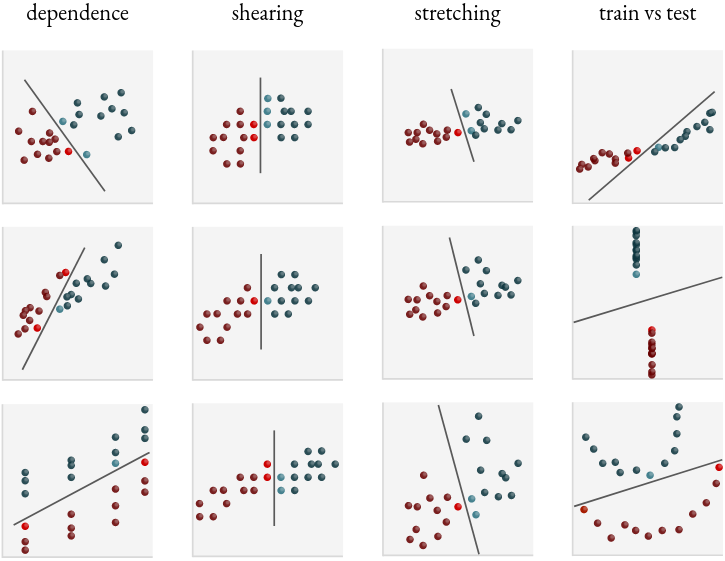
\includegraphics[width=\textwidth]{feature-space-phenomena}
        \end{marginfigure}

        % dependence 
        Just because two features both correlate with a positive label ($y=+1$)
        doesn't mean both features will have positive weights.  In other words,
        it could be that the \emph{blah}-feature correlates with $y=+1$ in the
        training set and yet, according to the best hypothesis for that
        training set, the bigger a fresh input's blah feature is, the
        \emph{less} likely its label is to be $+1$, all else being equal.  That
        last phrase ``all else being equal'' is crucial, since it refers to our
        choice of coordinates.
        %
        \attnsam{Illustrate `averaging' of good features vs `correction' of one
        feature by another (how much a feature correlates with error)}
        %
        In fact, t This is the difference between \emph{independence} and
        \emph{conditional independence}.

        % shearing
        Shearing two features together --- e.g.\ measuring
        cooktime-plus-preptime together with cooktime rather than preptime
        together with cooktime --- can impact the decision boundary.
        %
        Intuitively, the more stretched out a feature axis is, the more the
        learned hypothesis will rely on that feature.

        % stretching
        Stretching a single feature --- for instance, measuring it in
        centimeters instead of meters --- can impact the decision boundary
        as well.  Intuitively, the more stretched out a feature axis is, 
        the more the learned hypothesis will rely on that feature.

        % train vs test
        Note that

        %Caution: a feature $A(\sfx)$ that is statistically independent from
        %$\sfy$ may still be relevant for predicting $\sfy$.\marginnote{%
        %  Example.  Consider the uniform distribution on the four corners of a
        %  tetrahedron embedded within the corners of a cube \attnsam{TODO:
        %  graphic}.  The three spatial coordinates give three bit-valued random
        %  variables.  Any two of these variables are independent.  But the
        %  three together are dependent.
        %  \attnsam{TODO: also do a decision boundary (simpsons style) graph
        %  illustrating this phenomenon}
        %}
        %For example, if
        %$A, B$ are two features, it is possible that $A(\sfx), \sfy$ are
        %independent and that $B(\sfx), \sfy$ are independent and yet
        %$A(\sfx),B(\sfx), \sfy$ are \emph{dependent}!

        \attnsam{TODO: example featurization (e.g. MNIST again?)}


      \samsubsubsection{richer outputs}%larger $\yY$s} % $k$-ary classification; regression; probabilities
        We've learned how to construct a set $\hH$ of candidate patterns 
        $$
          f_{\vec w}(\vec x) = \text{step}(\vec w\cdot \vec x) 
        $$
        that map (a featurization of) a prompt $\vec x$ to a binary answer $y=0$ or $y=1$.

        What if we're interested in predicting a richer kind of $y$?  For
        example, maybe there are $k$ many possible values for $y$ instead of
        just $2$.  Or maybe there are infinitely many possible values --- say,
        if $y$ is a real number or a length-$l$ list of real numbers.  Or maybe we want the added nuance of
        predicting probabilities, so that $f$ might output ``20\% chance of
        label $y=0$ and 80\% chance of label $y=1$'' instead of just ``$y=1$''.

        I'll write formulas and then explain.
        $$
          f_{\vec w_i : 0\leq i < k}(\vec x) = \text{argmax}_i(\vec w_i\cdot \vec x) 
        $$
        $$
          f_{\vec w}(\vec x) = \vec w \cdot \vec x
        $$
        \attnsam{TODO: add multi-output regression?}
        $$
          f_{\vec w_i  : 0\leq i < k}(\vec x) = \text{normalize}(\exp(\vec w_i \cdot \vec x) : 0\leq i < k)
        $$
        \attnsam{TODO: interpret}

        \attnsam{TODO: discuss measures of goodness!}

        \attnsam{TODO: talk about structured (trees/sequences/etc) output!}


    \newpage
    \samsubsection{iterative optimization} 
      \samquote{
        Hey Jude, don't make it bad \\
        Take a sad song and make it better \\
        Remember to let her under your skin \\
        Then you'll begin to make it \\
        Better, better, better, better, better, better, ...
      }{paul mccartney, john lennon}

      \samsubsubsection{(stochastic) gradient descent}
        We have a collection $\hH$ of candidate patterns together with a
        function $1-\Ein$ that tells us how good a candidate is.\marginnote{%
          $\leftarrow$ We view $1-\Ein$ as an estimate of our actual notion of ``good'': $1-\Eout$.
        }
        %
        In \S A we found a nearly best candidate by brute-force search over all of
        $\hH$; this doesn't scale to the general case, where $\hH$ is
        intractably large.
        %
        So: \emph{what's a faster algorithm to find a nearly best candidate?}

        A common idea is to start arbitrarily with some $h_0\in \hH$ and
        repeatedly improve to get $h_1, h_2, \cdots$.  Two questions are:
        \emph{how do we select $h_{t+1}$ in terms of $h_t$}?  And \emph{how do
        we know when to stop}?  We'll discuss termination conditions later
        --- for now, let's agree to stop at $h_{10000}$.   

        As for selecting a next candidate, we'd like to use more detailed
        information on $h_t$'s inadequacies to inform our proposal $h_{t+1}$.
        Intuitively, if $h_t$ misclassifies a particular $(x_n, y_n) \in \sS$,
        then we'd like $h_{t+1}$ to be like $h_t$ but nudged a bit in the
        direction of accurately classifying $(x_n, y_n)$.

        %
        \attnsam{FILL IN FOR PROBABILITIES (LOGISTIC) MODEL} 

        This is the idea of \textbf{gradient descent}.
        \attnsam{MOTIVATE AND GIVE PSEUDOCODE FOR STOCHASTIC GD} 

        Given a list of training examples, a probability model, and a
        hypothesis $\vec w$, we can compute $\vec w$'s asserted probability
        that the training $x$s correspond to the training $y$s.  It's
        reasonable to choose $\vec w$ so that this probability is maximal.
        This method is called \textbf{maximum likelihood estimation (MLE)}.
        
      \samsubsubsection{logistic models} %``soft''

        The probability of a bunch of independent observations is the same as
        the product of probabilities of the observations.  Taking logarithms
        turns products into more manageable sums.  And --- this is a historical
        convention --- we further flip signs $\pm$ to turn maximization to 
        minimization.
        %
        After this translation, MLE with the logistic model means finding $\vec
        w$ that minimizes
        $$
          \sum_i \log(1+\exp(-y_i\vec w\cdot \vec x_i))
          =
          \sum_i \text{softplus}(-y_i\vec w\cdot \vec x_i) 
        $$
        Here, $\text{softplus}$ is our name for the function that sends
        $z$ to $\log(1+\exp(z))$.

        %We get a crucial-in-history and intuition-pumping-in-modern-times
        %algorithm when we do logistic regression in the limit of low
        %temperatures.  Perceptrons.

        \attnsam{mention convexity and convergence?}
        \attnsam{show trajectory in weight space over time -- see how certainty degree of freedom is no longer redundant? (``markov'')}

      \newpage
      \samsubsubsection{humble models}
        %Logistic ain't the only way to go.
        Let's generalize logistic classification to allow for \emph{unknown
        unknowns}. We'll do this by allowing a classifier to distribute
        probability mass not only among the labels $\yY$ but also to a special
        class $\star$ that means ``no comment'' or ``alien input''.  
        A logistic classifier always sets
        $\Pp_{\sfy|\sfx}[\star|x] = 0$.
        %
        But we could use other probability models that put nonzero mass on ``no
        comment''; different models give different learning programs.  Here are
        four models we might try:
        \newcommand{\zp}{u^{\!+\!}}
        \newcommand{\zm}{u^{\!-\!}}
        \begin{table}
          \centering
          \small
          \vspace{-0.3cm}
          \begin{tabular}{RCCCC}
                                        & \textsc{logistic}     & \textsc{perceptron}       & \textsc{svm}              & \textsc{gauss-gen}        \\\hline %& \textsc{gauss}                
            \Pp_{\sfy|\sfx}[-1| x]      & \zm/(\zm+\zp)         &\zm\cdot(\zm\wedge\zp)/2   &\zm\cdot(\zm/e\wedge\zp)/2 &\zm\cdot\text{bumps}       \\       %&\zm \cdot \epsilon e^{-d^2/4}  
            \Pp_{\sfy|\sfx}[+1| x]      & \zp/(\zm+\zp)         &\zp\cdot(\zm\wedge\zp)/2   &\zp\cdot(\zm\wedge\zp/e)/2 &\zp\cdot\text{bumps}       \\       %&\zp \cdot \epsilon e^{-d^2/4}  
            \Pp_{\sfy|\sfx}[\star| x]   & 1 - ~\text{above}=0   &1 - ~\text{above}          &1 - ~\text{above}          &1 - ~\text{above}          \\\hline %&1 - ~\text{above}               
            %                                                                                                                                                %                                
            \text{loss name}            &\text{softplus}(\cdot) &\text{srelu}(\cdot)        &\text{hinge}(\cdot)        &\text{quad}(\cdot)         \\       %&\text{parab}(\cdot)            
            \text{formula}              &\log(1+\exp(\cdot))    &\max(1,\cdot)+1            &\max(1,\cdot+1)            & ??                        \\       %&(\cdot+1)^2                    
            \text{update}               &1/(1+\exp(+yd))        &\text{step}(-yd)           &\text{step}(1-yd)          & ??                        \\\hline %&2(1-yd)                        
            %                                                                                                                                                %                                
            \text{outliers}             &\text{vulnerable}      &\text{robust}              &\text{robust}              &\text{vulnerable}          \\       %&\text{vulnerable}              
            \text{inliers}              &\text{sensitive}       &\text{blind}               &\text{sensitive}           &\text{blind}               \\       %&\text{blind}                   
            \text{humility}             &\text{low}             &\text{low}                 &\text{high}                &\text{high}                   
            %\text{humility}             &\text{low}             &\text{medium}              &\text{high}                \\             % &\text{high}                   
            %\text{acc bnd}              &\text{good}            &\text{bad}                 &\text{good}                \\             % &\text{medium}                 
            % TODO: split outliers/inliers by good or bad (erroneously classified or not?)  so 4 rows instead of 2?
          \end{tabular}
          \caption{%
            \textbf{Four popular models for binary classification.}
            %
            \textbf{Top rows:} Modeled chance given $x$ that $y=+1$ or $-1$ or
            $\star$.  We use $d = \vec w\cdot \vec x$, $u^{\!\pm\!}$ =
            $e^{\!\pm\! d/2}$, $a\wedge b = \min(a,b)$ to save ink.  And
            $\text{bumps}=(\phi(d-1)+\phi(d+1))/2$ with $\phi(\cdot)$ the
            standard normal density function.
            %
            \textbf{Middle rows:} neg-log-likelihood losses.
            %that arise when maximize likelihood using these models.
            An SGD step looks like
            $
              \vec w_{t+1} = \vec w_t + (\eta \cdot \text{update} \cdot y \vec x)
            $.
            %
            \textbf{Bottom rows:} All models respond to misclassifications.
            But are they robust
            to well-classified outliers?
            Sensitive to well-classified inliers?
            \par\noindent
            \attn{Exercise}: {
               Fill in the ??s in the rightmost column of the table above.
            }
          }
          \vspace{+0.3cm}
        \end{table}

        MLE with the perceptron model, svm model, or gauss-gen model minimizes
        the same thing, but with
        $\text{srelu}(z) = \text{max}(0,z)+1$,
        $\text{hinge}(z) = \text{max}(0,z+1)$, or
        $\text{quad}(z) = \cdots$
        instead of $\text{softplus}(z)$.\bcirc\marginnote{%
          \blarr Other models we might try will induce other substitutes for softplus.
          E.g.  $z\mapsto \text{hinge}(z)^2$ or $z\mapsto
          \text{avg}(z, \sqrt{z^2+4})$. 
        }
        %https://www.desmos.com/calculator/3yak0ozell

        Two essential properties of $\text{softplus}$ are that:
        (a) it is convex and
        (b) it upper bounds the step function. 
        Note that $\text{srelu}$, $\text{hinge}$, and $\text{quad}$ also enjoy
        these properties.  Property (a) ensures that the optimization problem
        is relatively easy --- under mild conditions, gradient descent is
        guaranteed to find a global minimum.  By property (b), the total loss
        on a training set upper bounds the rate of erroneous classification on
        that training set.  So loss is a \emph{surrogate} for (in)accuracy: if
        the minimized loss is nearly zero, then the training accuracy is nearly
        $100\%$.\marginnote{%
          The perceptron satisfies (b) in a trivial way that yields a trivial
          bound of $100\%$ on the error rate.
        }

        \attnsam{training behavior!!}
        \attnsam{response to outliers}
        \attnsam{support vectors}

      \samsubsubsection{ideas in stochastic gradient descent}
        \attn{learning rate as metric; robustness to 2 noise structures}
        \attn{nesterov momentum}
        \attn{decaying step size; termination conditions}
        \attn{batch normalization}

    \newpage
    \samsubsection{priors and generalization} 
      \samquote{
        A child's education should begin at least 100 years before [they are]
        born.
      }{oliver wendell holmes jr}
      %\samquote{
      %  I believe that either Jupiter has life or it doesn't.
      %  But I neither believe that it does, nor do I believe that it doesn't.
      %}{raymond smullyan}

      \samsubsubsection{on overfitting}
        \attnsam{$\Ee$ and $\max$ do not commute}
        \attnsam{point estimates vs bayesian decision theory}
        \attnsam{interpolation does not imply overfitting}

      \samsubsubsection{log priors and bayes}
        \attnsam{fill in computation and bases}
        \attnsam{visual illustration of how choice of L2 dot product matters}
        \attnsam{$\ell^p$ regularization; sparsity}
        \attnsam{eye regularization example!}

      \samsubsubsection{hierarchy, mixtures, transfer} 
        \attnsam{k-fold cross validation}
        \attnsam{dimension-based generalization bound}
        \attnsam{bayesian information criterion}

      \samsubsubsection{estimating generalization} 
        \attnsam{k-fold cross validation}
        \attnsam{dimension-based generalization bound}
        \attnsam{bayesian information criterion}


  \newpage
  \samsection{G. math refresher}
    \samsubsection{linear algebra}
        Linear algebra is the part of geometry that focuses on %the notions of
        when a point is the origin, when a `line' is a straight, and when two
        straight lines are parallel.
        %
        Linear algebra thus helps us deal with the preceding pictures
        %\marginnote{%
        %  $\leftarrow$ It is important to \attn{thoroughly understand these
        %  basics} of linear algebra.  Please see \S G.2 for further discussion
        %  of these basics. 
        %}
        mathematically and automatically.  The concept of `straight lines'
        gives a simple, flexible model for extrapolation from known points to
        unknown points.  That is intuitively why linear algebra will be crucial
        at every stage of 6.86x.

      \samsubsubsection{column vectors and row vectors} % vectors and co-vectors
        The elements of linear algebra are \textbf{column vectors} and
        \textbf{row vectors}.\bcirc \marginnote{%
          \blarr Though we represent the two similarly in a computer's memory, they
          have different geometric meanings.  We save much anguish by
          remembering the difference.
        }
        We have a set $V$ of ``column vectors''.  We're allowed to find $V$'s
        zero vector and to add or scale vectors in $V$ to get other vectors in
        $V$.  $V$ is the primary object we hold in our mind; perhaps, if we're
        doing image classification, then each column vector represents a
        photograph.  We use the word ``space'' or ``vector space'' when talking
        about $V$ to emphasize that we'd like to exploit visual intuitions when
        analyzing $V$.  In short: we imagine each column vector as a point in
        space, or, if we like, as an arrow from the zero vector to that point.
        
        Now, associated to $V$ is the set of ``row vectors''.  Under the hood, a
        row vector is a linear function from $V$ to the real numbers $\Rr$.  We
        imagine each row vector not as an arrow but as a ``linear'' heat map or
        altitude map that assigns to each point in $V$ a numeric ``intensity''.
        We can visualize a row vector the same way makers of geographic maps
        do: using contours for where in $V$ the row vector attains values
        $\cdots,-2,-1,0,+1,+2,\cdots$.
        These will be a bunch of uniformly spaced parallel ``planes''.  The
        spacing and orientation of the planes depends on and determines the row
        vector.  In short, we imagine each row vector as a collection of
        parallel planes in space.

        Informally: a column vector is a noun or thing whereas a row vector is
        a adjective or property.  The degree to which a property holds on a
        thing (or a description is true of a thing) is gotten by evaluating the
        row vector on the column vector --- remember, a row vector is a
        function, so we can do this evaluation.  Geometrically, if a row vector
        is a bunch of planes and a column vector is an arrow, the two evaluate
        to a number: the number of planes that the arrow pierces.  Intuitively,
        an example of a column vector might be ``this particular photo of my
        pet cow''; an example of a row vector might be ``redness of the left
        half (of the input photo)''.  If we evaluate this row vector on this
        column vector, then we get a number indicating how intensely true it is
        that the left half of that particular photo is red.\marginnote{%
            We can draw an analogy with syntax vs semantics.  This pair of
            concepts pops up in linguistics, philosophy, circuit engineering,
            quantum physics, and more, but all we need to know is that:
            semantics is about things while syntax is about descriptions of
            things.  The two concepts relate in that, given a set of things, we
            can ask for the set of all descriptions that hold true for all
            those things simultaneously.  And if we have a set of descriptions,
            we can ask for the set of all things that satisfy all those
            descriptions simultaneously.  These two concepts stand in formal
            opposition in the sense that: if we have a set of things and make
            it bigger, then the set of descriptions that apply becomes smaller.
            And vice versa.  Then a column vector is an object of semantics.
            And a row vector is an object of syntax.
        }
        
      \samsubsubsection{inner products}
        Now, here is the key point: the engine behind generalization in machine
        learning (at least, the machine learning we'll do in Units 1 and 2; and
        less visibly but still truly in more than half of each of Units 3,4,5)
        is the ability to translate between things and properties.  If ``my pet
        cow'' is a thing, then ``similar to my pet cow'' is a property.  The whole
        project of machine learning is to define and implement this word
        ``similar to''.  When we define and implement well, our programs can
        generalize successfully from training examples to new, previously
        unseen situations, since they will be able to see which of the training
        examples the new situations are similar to.  Since ``similar to''
        transforms things to properties, the linear algebra math behind
        ``similar to'' is a function from column vectors to row vectors.  This
        brings us to...

        ... inner products, aka kernels.  An inner product is just a fancy word
        for a (linear) function from column vectors to row vectors.  We
        actually demand that this linear function has two nice properties:
        FIRST, it should have an inverse.  That is, it ought to be a two way
        bridge between column vectors and row vectors, allowing us to translate
        things to descriptions and vice versa.  SECOND, it should be symmetric.
        This means that if we have two things, say ``my pet cow'' and ``my pet
        raccoon'', then the degree to which ``my pet raccoon'' has the property
        ``is similar to my pet cow'' ought to match the degree to which ``my pet
        cow'' has the property ``is similar to my pet raccoon''.  Any invertible,
        symmetric, linear function from column vectors to row vectors is called
        an inner product.  Kernel is a synonym here.\marginnote{%
          Beware: the same word, ``kernel'', has different meanings depending
          on context.
        }

        There are generally infinitely many inner products.  Which one we
        choose changes the generalization properties of our machine learning
        program.  Practically, if we are doing machine learning in a concrete
        situation, then we want to choose an inner product that reflects our
        human intuition and experience and domain knowledge about the right
        notion of ``similarity'' in that situation.
        
        Any inner product $P$ from column vectors to row vectors induces notions
        of length and angle.  We just define a column vector v's length by
        $\sqrt{P(v)(v)}$.  Call that quantity $\|v\|$.  And we define the angle
        $\alpha(v,w)$ between two non-zero column vectors v,w by
        $P(v)(w)=\|v\|\cdot\|w\|\cdot\cos\alpha(v,w)$.  We make these
        definitions so as to match the Pythagorean theorem from plane geometry.\marginnote{%
          You can google up proofs of the Pythagorean theorem (many are quick and
          beautiful) if you wish to dig deeper.  
        }
        So once we choose which inner product we'll use (out of the infinitely
        many choices), we get the concepts of euclidean geometry for free.
        Immediately following from that definition of angle, we get that if two
        column vectors have vanishing inner product (i.e., if $P(v)(w)=0$), then
        those vectors are at right angles (i.e. $\alpha(v)(w)=\pi/2$).
        
        Now, sometimes (but most of the time not), we are blessed in
        that we know more about our situation than just the space V of things.
        Specifically, V might come with a canonical basis.  This just means
        that V comes marked with "the right" axes with respect to which we
        ought to analyze vectors in V.  In this fortunate case, there is also a
        canonical inner product.  It's called dot product.  Again, I want to
        emphasize that a plain vector space doesn't come with a dot product.
        We need a basis for that.

        %The dot product is defined as follows.  Say there are D axes and that
        %the "unit" vectors along each axis (aka the basis vector) are named
        %(vi:0≤i<D).  Then we define P(vj)(vi)=1 if i=j else 0 --- the 1
        %expresses that each "unit" basis vector ought to have length 1.  The 0
        %expresses that different basis vectors ought to be at right angles to
        %each other.  This determines P on all inputs, by linearity:
        %P(∑c′jvj)(∑civi)=∑ic′ici where c′j,ci are numbers.  In short: given a
        %basis, there is a unique inner product such that those basis elements
        %all have length 1 and are at right angles to each other.  We call that
        %inner product the dot product.

        \attnsam{FILL IN LINEAR DECISION BOUNDARY! (remark on featurization and
        argmax nonlinearities)}

        We may \textbf{evaluate} a row vector on a column vector.  \attnsam{FILL
        IN} A \textbf{dot product} is a way of translating between row and
        column vectors.  \attnsam{FILL IN: DISCUSS GENERALIZATION; (DISCUSS ANGLE, TOO)}

\end{document}

